\section{Rigid Body Transformations}

A vehicle moves in space and carries many sensors, each with its own reference frame.
To describe its motion, and to combine the measurements of different sensors, we need a precise mathematical description of positions, orientations and changes of reference frame: the \textbf{rigid body transformations}.

\subsection{Rigid bodies and rigid transformations}
A \textbf{rigid body} is an object whose shape and size do not change, even when forces act on it: it does not bend, stretch or compress, and every pair of its points stays at the same distance.
A rigid body can move in only two ways: \textbf{translation} (the whole body moves from one place to another) and \textbf{rotation} (the body spins about an axis).
Vehicles can be considered rigid bodies.

A \textbf{rigid body transformation} is a transformation that preserves shape and size, changing only the position and the orientation of the body. It is made of a translation, which moves the object, and a rotation, which changes its orientation.
The movement of a vehicle can be seen as the result of a sequence of rigid body transformations.

\subsection{Translation}
A translation is represented by a vector $t = [t_x, t_y, t_z]^T$ and moves every point by the same offset: $p' = p + t$.
Using homogeneous coordinates (we add a fourth coordinate equal to 1) we can write it as a matrix product:
\[
p' = \begin{bmatrix} 1 & 0 & 0 & t_x \\ 0 & 1 & 0 & t_y \\ 0 & 0 & 1 & t_z \\ 0 & 0 & 0 & 1 \end{bmatrix} p
\]
This is the reason why homogeneous coordinates are so convenient: rotations and translations become both matrix products, and they can be combined into a single matrix.

\subsection{Rotations}
Rotations can be represented in three main ways: Euler angles, rotation matrices and quaternions.

\subsubsection{Euler angles}
The rotation is represented as three successive rotations about the coordinate axes, with the angles \textbf{roll} ($\phi$), \textbf{pitch} ($\theta$) and \textbf{yaw} ($\psi$):
\[
R = R_x(\phi)\,R_y(\theta)\,R_z(\psi) =
\begin{bmatrix} 1 & 0 & 0 \\ 0 & \cos\phi & -\sin\phi \\ 0 & \sin\phi & \cos\phi \end{bmatrix}
\begin{bmatrix} \cos\theta & 0 & \sin\theta \\ 0 & 1 & 0 \\ -\sin\theta & 0 & \cos\theta \end{bmatrix}
\begin{bmatrix} \cos\psi & -\sin\psi & 0 \\ \sin\psi & \cos\psi & 0 \\ 0 & 0 & 1 \end{bmatrix}
\]
Euler angles are \textbf{intuitive} (close to how humans describe an orientation) and \textbf{compact} (only 3 parameters).
However, the representation is \textbf{discontinuous} (the angles can suddenly jump, e.g.\ from $180^\circ$ to $-180^\circ$), the same rotation has \textbf{multiple equivalent representations}, and \textbf{interpolating} between two orientations is difficult and unintuitive.

\subsubsection{Rotation matrices}
A rotation can be represented by a matrix $R$ belonging to the \textbf{special orthogonal group}:
\[
SO(3) = \{ R \in \mathbb{R}^{3\times3} \mid R \text{ is orthogonal},\ \det(R) = 1 \}
\]
Rotation matrices preserve lengths and angles, and they are used in robotics, physics and computer graphics.
For example, the rotation about the $z$ axis is:
\[
R_z(\theta) = \begin{bmatrix} \cos\theta & -\sin\theta & 0 \\ \sin\theta & \cos\theta & 0 \\ 0 & 0 & 1 \end{bmatrix}
\]
Since $R$ is orthogonal, its inverse is simply its transpose: $R^{-1} = R^T$.

\subsubsection{Quaternions}
A \textbf{quaternion} is written as
\[
q = w + xi + yj + zk, \qquad w, x, y, z \in \mathbb{R}, \qquad i^2 = j^2 = k^2 = ijk = -1
\]
and \textbf{unit quaternions} ($\|q\| = 1$) represent 3D rotations.
With respect to the other representations they are \textbf{compact} (4 numbers instead of the 9 of a matrix), they have \textbf{no gimbal lock} and they allow an efficient \textbf{interpolation} (slerp). They can be converted to and from rotation matrices, and they are widely used in 3D graphics, animation and robotics.

The main operations are:
\[
\|q\| = \sqrt{w^2 + x^2 + y^2 + z^2} \qquad\quad
q^* = w - xi - yj - zk \qquad\quad
q^{-1} = \frac{q^*}{\|q\|^2}
\]
The \textbf{multiplication} of quaternions corresponds to the \textbf{composition} of rotations and, like matrix multiplication, it is not commutative.

To \textbf{rotate a vector} $v = (v_x, v_y, v_z)$ we write it as a pure quaternion, $\hat{v} = 0 + v_x i + v_y j + v_z k$, and, given a unit quaternion $q$, the rotated vector is
\[
\hat{v}' = q\,\hat{v}\,q^{-1}
\]
This preserves the length ($\|v'\| = \|v\|$) and it is equivalent to applying the rotation matrix derived from $q$.

\begin{infobox}[Gimbal lock]
With Euler angles, when the middle rotation reaches $\pm 90^\circ$ (e.g.\ pitch $= 90^\circ$), the first and the third rotation axes become aligned: one degree of freedom is lost, and different combinations of roll and yaw produce the same orientation. This is called \textbf{gimbal lock}, and it is one of the main reasons why quaternions are preferred to represent orientations.
\end{infobox}

\subsection{The special Euclidean group SE(3)}
The set of all rigid body transformations in 3D is the \textbf{special Euclidean group}, which combines a rotation $R$ and a translation $t$ into a single $4\times4$ matrix:
\[
SE(3) = \left\{ \begin{bmatrix} R & t \\ 0 & 1 \end{bmatrix} \ \middle|\ R \in SO(3),\ t \in \mathbb{R}^3 \right\}
\]
It has a \textbf{group structure}: the composition of two transformations is still a transformation, the identity is $\begin{bmatrix} I_3 & 0 \\ 0 & 1 \end{bmatrix}$, and every transformation has an inverse:
\[
\begin{bmatrix} R & t \\ 0 & 1 \end{bmatrix}^{-1} = \begin{bmatrix} R^T & -R^T t \\ 0 & 1 \end{bmatrix}
\]
Note that the translation must be \textbf{rotated} before being negated: the inverse is not simply $-t$.

\begin{examplebox}[Applying SE(3) to a point]
A point in homogeneous coordinates is $p = [x, y, z, 1]^T$, and a rigid transformation is applied as $p' = Tp$.
For example, a rotation about $z$ by $\theta$ followed by a translation $(1, 2, 0)$ is
\[
T = \begin{bmatrix} \cos\theta & -\sin\theta & 0 & 1 \\ \sin\theta & \cos\theta & 0 & 2 \\ 0 & 0 & 1 & 0 \\ 0 & 0 & 0 & 1 \end{bmatrix}
\]
\end{examplebox}

\subsubsection{Twists}
A \textbf{twist} compactly represents the \textbf{instantaneous velocity} of a rigid body:
\[
\xi = \begin{bmatrix} v \\ \omega \end{bmatrix} \in \mathbb{R}^6
\]
where $v \in \mathbb{R}^3$ is the linear velocity and $\omega \in \mathbb{R}^3$ the angular velocity.

\subsection{Reference frames}
A \textbf{reference frame} is a coordinate system with an origin and three axes.
A \textbf{sensor reference frame} is fixed to the sensor: its origin is typically at the centre of the sensor (the camera lens, the IMU, the LiDAR centre) and its axes are defined by the sensor orientation (e.g.\ x-right, y-down, z-forward for a camera).
All the measurements of a sensor are expressed in its own frame, so, for \textbf{sensor fusion}, they must first be transformed into a \textbf{common reference frame}.

\begin{figure}[H]
    \centering
    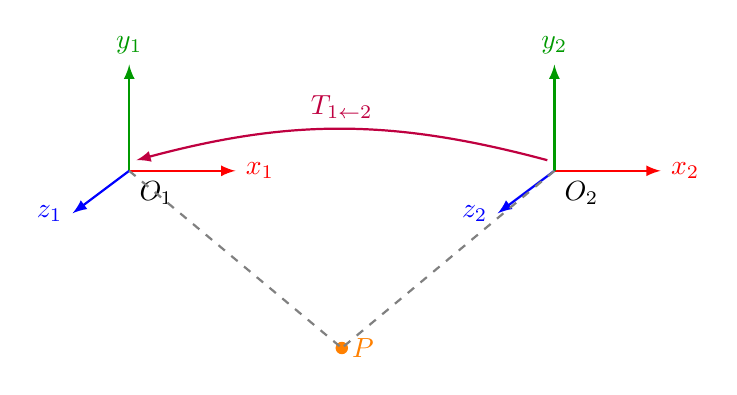
\begin{tikzpicture}[scale=0.9, >=latex, thick]
        % frame 1
        \draw[->, red] (0,0) -- (1.5,0) node[right] {$x_1$};
        \draw[->, green!60!black] (0,0) -- (0,1.5) node[above] {$y_1$};
        \draw[->, blue] (0,0) -- (-0.8,-0.6) node[left] {$z_1$};
        \node[below right] at (0,0) {$O_1$};
        % frame 2
        \draw[->, red] (6,0) -- (7.5,0) node[right] {$x_2$};
        \draw[->, green!60!black] (6,0) -- (6,1.5) node[above] {$y_2$};
        \draw[->, blue] (6,0) -- (5.2,-0.6) node[left] {$z_2$};
        \node[below right] at (6,0) {$O_2$};
        % transform
        \draw[->, purple] (5.9,0.15) to[bend right=15] node[midway, above] {$T_{1\leftarrow2}$} (0.1,0.15);
        % point
        \fill[orange] (3,-2.5) circle (2.5pt) node[right] {$P$};
        \draw[dashed, gray] (0,0) -- (3,-2.5);
        \draw[dashed, gray] (6,0) -- (3,-2.5);
    \end{tikzpicture}
    \caption{The same point $P$ seen from two sensor frames: $p_1 = [2, 4, -2]$, $p_2 = [-3, 4, -2]$, and there exists $T_{1\leftarrow2} \in SE(3)$ such that $p_1 = T_{1\leftarrow2}\,p_2$}
\end{figure}

\subsubsection{Changing the reference frame of a point}
A point can be expressed in different coordinate frames. If $p_B$ are its coordinates in frame $B$ and $T_{A\leftarrow B} \in SE(3)$ is the transformation from frame $B$ to frame $A$, then
\[
p_A = T_{A\leftarrow B}\, p_B, \qquad
T_{A\leftarrow B} = \begin{bmatrix} R_{A\leftarrow B} & t_{A\leftarrow B} \\ 0 & 1 \end{bmatrix}
\]
where $R_{A\leftarrow B} \in SO(3)$ says how frame $B$ is rotated with respect to frame $A$, and $t_{A\leftarrow B} \in \mathbb{R}^3$ says where the origin of $B$ is with respect to the origin of $A$.
For example, to convert a point seen by camera 2 into the frame of camera 1: $p_1 = T_{1\leftarrow2}\,p_2$.

To go back we use the inverse, which is exactly the transformation in the opposite direction:
\[
T_{A\leftarrow B}^{-1} = \begin{bmatrix} R^T & -R^T t \\ 0 & 1 \end{bmatrix} = T_{B\leftarrow A},
\qquad p_B = T_{A\leftarrow B}^{-1}\, p_A = T_{B\leftarrow A}\, p_A
\]

\begin{infobox}[Reading the notation]
The notation $T_{A\leftarrow B}$ is read from right to left: it takes a point expressed in $B$ and returns it in $A$. This makes chains easy to check, since the inner indices must match: $T_{A\leftarrow C} = T_{A\leftarrow B}\, T_{B\leftarrow C}$.
\end{infobox}

\subsubsection{Changing the reference frame of a twist}
A twist also depends on the frame in which it is expressed. If $\xi_B$ is expressed in frame $B$, to express it in frame $A$ we use the \textbf{adjoint transformation} of SE(3):
\[
\xi_A = \mathrm{Ad}_{T_{A\leftarrow B}}\, \xi_B, \qquad
\mathrm{Ad}_T = \begin{bmatrix} R & [t]_\times R \\ 0 & R \end{bmatrix} \in \mathbb{R}^{6\times6}
\]
where $R$ is the rotation from $B$ to $A$, $t$ the translation, and $[t]_\times$ is the \textbf{skew-symmetric matrix} of $t$:
\[
[t]_\times = \begin{bmatrix} 0 & -t_z & t_y \\ t_z & 0 & -t_x \\ -t_y & t_x & 0 \end{bmatrix}
\]
which represents the cross product: $[t]_\times\, a = t \times a$.
The adjoint ensures that the angular and the linear velocity are transformed consistently: the angular velocity is simply rotated, while the linear velocity also gets the contribution of the rotation around the displaced origin ($t \times \omega$).

\subsection{Coordinate conventions}
\subsubsection*{FLU (vehicles)}
The \textbf{FLU} convention (Front--Left--Up) is commonly used in autonomous vehicles and drones:
\begin{compactitemize}
    \item $x$ points \textbf{forward}, in the direction of motion;
    \item $y$ points to the \textbf{left};
    \item $z$ points \textbf{up}.
\end{compactitemize}
It is a right-handed system, used for vehicle poses, sensor data and control commands.

\subsubsection*{RDF (cameras)}
The \textbf{RDF} convention (Right--Down--Front) is widely used in computer vision and camera models:
\begin{compactitemize}
    \item $x$ points to the \textbf{right} of the image plane;
    \item $y$ points \textbf{down} in the image plane;
    \item $z$ points \textbf{forward}, along the optical axis.
\end{compactitemize}

\begin{figure}[H]
    \centering
    \begin{subfigure}[b]{0.45\textwidth}
        \centering
        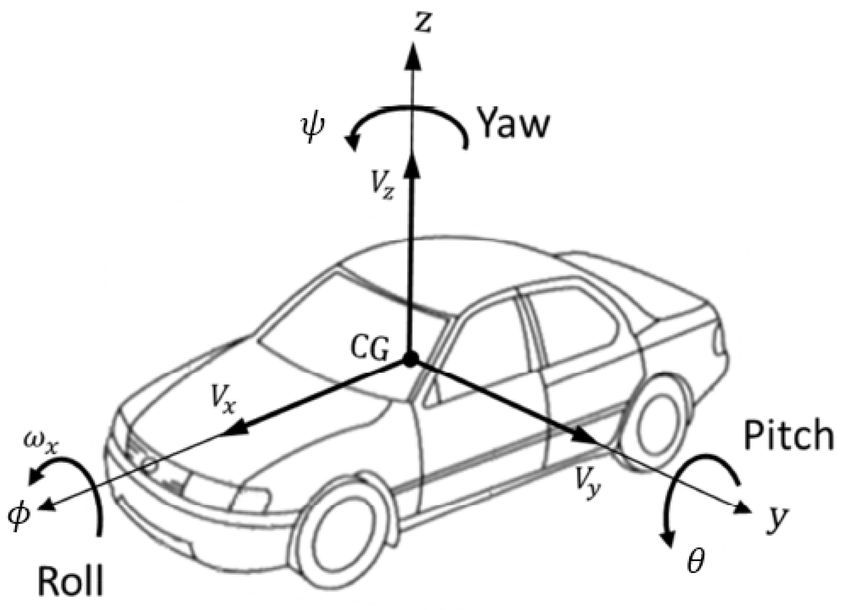
\includegraphics[height=4.2cm]{images/C7_1.png}
        \caption{FLU frame of a vehicle}
    \end{subfigure}
    \hfill
    \begin{subfigure}[b]{0.5\textwidth}
        \centering
        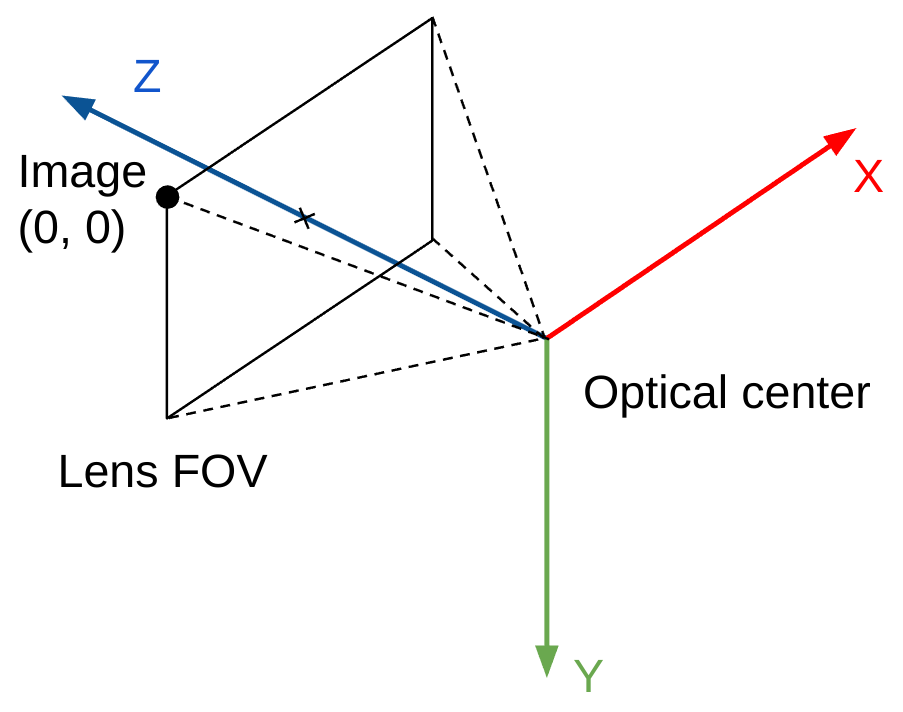
\includegraphics[width=\linewidth,height=4.2cm,keepaspectratio]{images/C7_2.png}
        \caption{RDF frame of a camera}
    \end{subfigure}
    \caption{The FLU and RDF coordinate conventions}
\end{figure}

\subsubsection{Conversion between FLU and RDF}
The two conventions are related by a pure rotation:
\[
\begin{bmatrix} x_{RDF} \\ y_{RDF} \\ z_{RDF} \end{bmatrix} = R_{RDF\leftarrow FLU} \begin{bmatrix} x_{FLU} \\ y_{FLU} \\ z_{FLU} \end{bmatrix}, \qquad
R_{RDF\leftarrow FLU} = \begin{bmatrix} 0 & -1 & 0 \\ 0 & 0 & -1 \\ 1 & 0 & 0 \end{bmatrix}
\]
Each row says where a camera axis comes from: right is minus left ($x_{RDF} = -y_{FLU}$), down is minus up ($y_{RDF} = -z_{FLU}$) and front is front ($z_{RDF} = x_{FLU}$).
Its inverse, i.e.\ its transpose, converts back:
\[
R_{FLU\leftarrow RDF} = R_{RDF\leftarrow FLU}^T = \begin{bmatrix} 0 & 0 & 1 \\ -1 & 0 & 0 \\ 0 & -1 & 0 \end{bmatrix}
\]
